\documentclass{standalone}
\usepackage{tikz}
\usepackage{ctex,siunitx}
\usepackage{tkz-euclide}
\usepackage{amsmath}
\usetikzlibrary{patterns, calc}
\usetikzlibrary {decorations.pathmorphing, decorations.pathreplacing, decorations.shapes,}
\begin{document}
\small
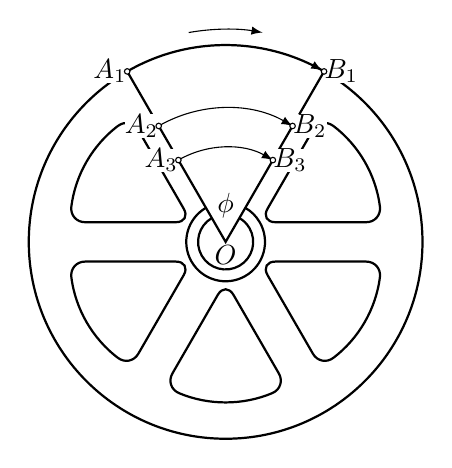
\begin{tikzpicture}[>=latex,scale=1.0,inner sep=0pt,fill=white]
  \draw[thick](0,0)circle(2.5);
  \foreach \x in {30,150,210,270,330}
  {
    \coordinate (A) at (\x:0.5);
    \coordinate (B) at ([shift=(\x-30:1.5513)]A);
    \coordinate (C) at ([shift=(\x+30:1.5513)]A);
    \draw[thick,rounded corners=2mm](A)--(B)to[bend right=22.8](C)--cycle;
  }
  \draw[thick](120:0.5)arc(120:420:0.5);
  \draw[thick](120:0.35)arc(120:420:0.35);
  \draw[thick](120:2.5)--(0,0)node[below,inner sep=1pt]{$O$}--(60:2.5);
  \draw[->](100:2.7)arc(100:80:2.7);
  \draw[->](120:1.2)node[left,fill]{$A_3$}arc(120:60:1.2)node[right,fill]{$B_3$};
  \draw[->](120:1.7)node[left,fill]{$A_2$}arc(120:60:1.7)node[right,fill]{$B_2$};
  \draw[decorate,decoration={markings,mark={at position 0.99 with{\arrow{>}}}}](120:2.5)node[left,fill]{$A_1$}arc(120:60:2.5)node[right,fill]{$B_1$};
  \fill[draw](120:1.2)circle(1pt)(120:1.7)circle(1pt)(120:2.5)circle(1pt)(60:1.2)circle(1pt)(60:1.7)circle(1pt)(60:2.5)circle(1pt);
  \node at (0,0)[above=3mm]{$\phi$};
\end{tikzpicture}
\end{document}